\documentclass[a4paper,11pt]{article}

% Kodovani (cestiny) v dokumentu: utf-8
%\usepackage[cp1250]{inputenc}	% Omezena stredoevropska kodova stranka, pouze MSW.
\usepackage[utf8]{inputenc}	% Doporucujeme pouzivat UTF-8 (unicode).

\usepackage[margin=2cm]{geometry}
\newtoks\jmenopraktika \newtoks\jmeno \newtoks\datum
\newtoks\obor \newtoks\skupina \newtoks\rocnik \newtoks\semestr
\newtoks\cisloulohy \newtoks\jmenoulohy
\newtoks\tlak \newtoks\teplota \newtoks\vlhkost

\jmenopraktika={Fyzikální praktikum 3}
\jmeno={Lukáš Lejdar}
\datum={26. února 2025}
\obor={F}
\skupina={Út 14:00}

\cisloulohy={8}
\jmenoulohy={Band gap width}

%%%%%%%%%%% Uzitecne balicky:

\usepackage{graphicx}
\usepackage{amsmath}
\usepackage{xspace}
\usepackage{url}
\usepackage{indentfirst}
\usepackage{wrapfig}
\usepackage{xcolor}
\usepackage{subfig}
\usepackage{subcaption}
\usepackage{enumitem}
\usepackage{tikzsymbols}
\usepackage{newfloat}

\DeclareFloatingEnvironment[fileext=lof]{graph}
\captionsetup[graph]{labelformat=simple, labelsep=colon, name=Graph}

%%%%%% Zamezeni parchantu:
\widowpenalty 10000 \clubpenalty 10000 \displaywidowpenalty 10000
%%%%%% Parametry pro moznost vsazeni vetsiho poctu obrazku na stranku
\setcounter{topnumber}{3}	  % max. pocet floatu nahore (specifikace t)
\setcounter{bottomnumber}{3}	  % max. pocet floatu dole (specifikace b)
\setcounter{totalnumber}{6}	  % max. pocet floatu na strance celkem
\renewcommand\topfraction{0.9}	  % max podil stranky pro floaty nahore
\renewcommand\bottomfraction{0.9} % max podil stranky pro floaty dole
\renewcommand\textfraction{0.1}	  % min podil stranky, ktery musi obsahovat text
\intextsep=8mm \textfloatsep=8mm  %\intextsep pro ulozeni [h] floatu a \textfloatsep pro [b] or [t]

% Tecky za cisly sekci:
\renewcommand{\thesection}{\arabic{section}.}
\renewcommand{\thesubsection}{\thesection\arabic{subsection}.}
% Jednopismenna mezera mezi cislem a nazvem kapitoly:
\makeatletter \def\@seccntformat#1{\csname the#1\endcsname\hspace{1ex}} \makeatother
%
\newcommand{\vsn}[4]{\ensuremath{#1 =} #2(#3)\,#4}
\newcommand{\vrn}[6]{\ensuremath{#1 =} (#2 $\pm$ #3)\,#4 ($p=$ #5\,\%, $\nu=$ #6)}

\newcommand*\circled[1]{\tikz[baseline=(char.base)]{
		\node[shape=circle,draw,inner sep=1pt] (char) {#1};}}

%%%%%%%%%%%%%%%%%%%%%%%%%%%%%%%%%%%%%%%%%%%%%%%%%%%%%%%%%%%%%%%%%%%%%%%%%%%%%%%
% Zacatek dokumentu
%%%%%%%%%%%%%%%%%%%%%%%%%%%%%%%%%%%%%%%%%%%%%%%%%%%%%%%%%%%%%%%%%%%%%%%%%%%%%%%

\begin{document}

\thispagestyle{empty}

{
\begin{center}
\sf 
{\Large Ústav fyziky a technologií plazmatu Přírodovědecké fakulty Masarykovy univerzity} \\
\bigskip
{\huge \bfseries FYZIKÁLNÍ PRAKTIKUM} \\
\bigskip
{\Large \the\jmenopraktika}
\end{center}

\bigskip

\sf
\noindent
\setlength{\arrayrulewidth}{1pt}
\begin{tabular*}{\textwidth}{@{\extracolsep{\fill}} l l}
\large {\bfseries Zpracoval:}  \the\jmeno & \large  {\bfseries Naměřeno:} \the\datum\\[2mm]
\large  {\bfseries Obor:} \the\obor  \hspace{40mm}  {\bfseries Skupina:} \the\skupina %
&\large {\bfseries Testováno:}\\
\\
\hline
\end{tabular*}
}

\bigskip

{
\sf
\noindent \begin{tabular}{p{4cm} p{0.6\textwidth}}
\Large  Úloha č. {\bfseries \the\cisloulohy:} \par
\smallskip
&\Large \bfseries \the\jmenoulohy  \\[2mm]
\end{tabular}
}

\vskip1cm

\section{Introduction}

An important characteristic of semiconductors is the band gap, influencing their electrical conductivity and optical properties. Our aim is to determine the band gap energy ($ E_{g} $ )  of silicon and germanium using the inner photoelectric effect.

\section{Theory}

Electrons bound to atoms can only exist at some discrete set of energy levels and to move around, they have to absorb or emit energy to keep it conserved. Both emission and absorption can happen via light, which is also discretized with photon particles. Each has an associated wavelength $ \lambda $ and it's energy  is given by

\begin{equation}
    E = \frac{h c}{\lambda}
\end{equation}

Semiconductors are special in that they have a certain energy gap $ E_g $ of banned states between it's electrons in the valance band and the conductive band. If we create a PN junction of these atoms and shine monochromatic light at it with increasing frequency, there comes a point where the photon energy exceeds the band gap $ E_g $. At this threshold, electrons jump to the conduction band, get carried by the junction's voltage, and a measurable voltage begins to build up.
 
\section{Measurement procedure}

The scheme of the experiment can be found in Figure $ 1 $. We have a source of white light shining into a monochromator, which is then directed onto the diode which has a connected voltmeter. To find the band gap energy $ E_g $, all we need to do is find the largest wavelength $ \lambda_{max} $, where the voltage starts to build up and plug into equation (1), to get

\begin{equation}
E_{g} = \frac{h c}{\lambda_{max}}
\end{equation}

\vspace{10pt}

We will then also proceed to measure the induced voltage for the whole spectrum. To do this, we also have to account for the fact, that our halogen lamp does not shine light with the same intensity at each wavelength. To correct for this, we have a table of values of relative intensity $ D(\lambda) $  emitted by lamp, and we will correct with

\begin{equation}
 S(\lambda) = \frac{U(\lambda)}{ D(\lambda) }
\end{equation}

As the last step, we will express each wavelength $ \lambda $ as energy of the photon $ E $ and plot the calculated function $ S(E) $.



\begin{figure}[htpb]
    \centering
    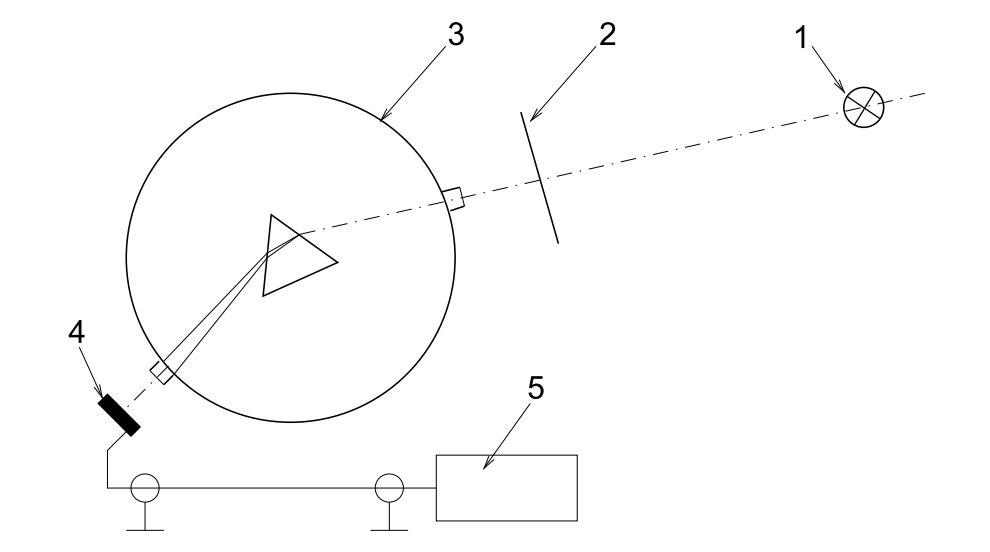
\includegraphics[width=0.65\textwidth]{aparatura.jpg}
    \caption{Scheme of the experiment: 1 - Halogen lamp, 2 - Convex lens, 3 - Monochromator, 4 - Semiconductor photodiode, 5 - Voltmetr}
\end{figure}


\section{Results}

We've measured one germanium diode and one made from silicon. The resulting voltages, as functions of wavelength, are presented in Table 1 and 2 and illustrated in Graphs 1 and 2. From these graphs, we can directly determine the maximum wavelengths $ \lambda_{max} $ and calculate the corresponding energy gaps using Equation (2).

\begin{table}[htpb]
    \centering
    \begin{tabular}{l c c}
        & $ \lambda_{max} $ (nm) & $ E_g $ (eV) \\ \hline
        silicon & 1160 & 1.069 \\
        germanium & 1930 &  0.642 \\ 
    \end{tabular}
\end{table}

\begin{table}[h]
    \scriptsize
    \centering
    \begin{tabular}{| c c c c | c c c c | c c c c | }
        \hline
        $ \lambda $ (nm) & $ U_m $ (mV) & $ E $ (eV) & $ S \cdot 10^{6} $ & $ \lambda $ (nm) & $ U_m $ (mV) & $ E $ (eV) & $ S \cdot 10^{6} $ & $ \lambda $ (nm) & $ U_m $ (mV) & $ E $ (eV) & $ S \cdot 10^{6} $ \\
        \hline
        0.792 & 0.03 & 1.56 & 0.14 & 1.154 & 0.58 & 1.07 & 4.27 & 1.525 & 0.46 & 0.81 & 4.45 \\
        0.853 & 0.06 & 1.45 & 0.31 & 1.160 & 0.57 & 1.06 & 4.24 & 1.550 & 0.42 & 0.79 & 4.19 \\
        0.879 & 0.09 & 1.41 & 0.49 & 1.175 & 0.57 & 1.05 & 4.27 & 1.575 & 0.42 & 0.78 & 4.31 \\
        0.899 & 0.12 & 1.37 & 0.67 & 1.200 & 0.62 & 1.03 & 4.69 & 1.600 & 0.36 & 0.77 & 3.90 \\
        0.914 & 0.15 & 1.35 & 0.86 & 1.225 & 0.67 & 1.01 & 5.19 & 1.625 & 0.33 & 0.76 & 3.70 \\
        0.925 & 0.18 & 1.34 & 1.05 & 1.250 & 0.72 & 0.99 & 5.70 & 1.650 & 0.32 & 0.75 & 3.75 \\
        0.942 & 0.21 & 1.31 & 1.25 & 1.275 & 0.74 & 0.97 & 5.88 & 1.675 & 0.27 & 0.74 & 3.37 \\
        0.960 & 0.24 & 1.29 & 1.46 & 1.300 & 0.77 & 0.95 & 6.22 & 1.680 & 0.24 & 0.73 & 3.04 \\
        0.975 & 0.27 & 1.27 & 1.67 & 1.325 & 0.78 & 0.93 & 6.44 & 1.700 & 0.20 & 0.72 & 2.68 \\
        0.985 & 0.30 & 1.25 & 1.88 & 1.350 & 0.75 & 0.91 & 6.29 & 1.725 & 0.21 & 0.71 & 3.04 \\
        1.000 & 0.33 & 1.23 & 2.11 & 1.362 & 0.69 & 0.91 & 5.83 & 1.750 & 0.17 & 0.70 & 2.62 \\
        1.015 & 0.36 & 1.22 & 2.34 & 1.375 & 0.66 & 0.90 & 5.63 & 1.775 & 0.20 & 0.69 & 3.62 \\
        1.030 & 0.39 & 1.20 & 2.57 & 1.400 & 0.63 & 0.88 & 5.49 & 1.800 & 0.19 & 0.68 & 3.79 \\
        1.045 & 0.42 & 1.18 & 2.81 & 1.425 & 0.70 & 0.87 & 6.15 & 1.825 & 0.15 & 0.67 & 3.64 \\
        1.061 & 0.45 & 1.16 & 3.06 & 1.450 & 0.75 & 0.85 & 6.76 & 1.850 & 0.10 & 0.67 & 2.93 \\
        1.075 & 0.48 & 1.15 & 3.31 & 1.475 & 0.72 & 0.84 & 6.63 & 1.875 & 0.08 & 0.66 & 3.17 \\
        1.092 & 0.51 & 1.13 & 3.57 & 1.485 & 0.66 & 0.83 & 6.14 & 1.900 & 0.05 & 0.65 & 3.89 \\
        1.107 & 0.54 & 1.11 & 3.83 & 1.500 & 0.60 & 0.82 & 5.69 & 1.930 & 0.01 & 0.64 & 7.35 \\
        1.130 & 0.57 & 1.09 & 4.12 & 1.515 & 0.54 & 0.81 & 5.18 &       &      &      &      \\
        \hline
    \end{tabular}
    \caption{Measured spectral photovoltage dependence of germanium diode.}
\end{table}

\begin{table}[h]
    \scriptsize
    \centering
    \begin{tabular}{| c c c c | c c c c |}
        \hline
        $ \lambda $ (nm) & $ U_m $ (mV) & $ E $ (eV) & $ S \cdot 10^{6} $ & $ \lambda $ (nm) & $ U_m $ (mV) & $ E $ (eV) & $ S \cdot 10^{6} $ \\
        \hline
        0.593 & 0.03 & 2.09 & 0.64 & 0.938 & 0.54 & 1.32 & 3.05 \\
        0.678 & 0.06 & 1.82 & 0.16 & 0.943 & 0.57 & 1.31 & 3.25 \\
        0.724 & 0.09 & 1.71 & 0.29 & 0.948 & 0.60 & 1.30 & 3.45 \\
        0.768 & 0.12 & 1.61 & 0.44 & 0.960 & 0.63 & 1.29 & 3.71 \\
        0.803 & 0.15 & 1.54 & 0.61 & 0.975 & 0.66 & 1.27 & 3.99 \\
        0.832 & 0.18 & 1.49 & 0.79 & 1.000 & 0.65 & 1.23 & 4.12 \\
        0.848 & 0.21 & 1.46 & 0.96 & 1.020 & 0.63 & 1.21 & 4.09 \\
        0.860 & 0.24 & 1.44 & 1.13 & 1.030 & 0.59 & 1.20 & 3.86 \\
        0.869 & 0.27 & 1.42 & 1.30 & 1.040 & 0.51 & 1.19 & 3.41 \\
        0.879 & 0.30 & 1.41 & 1.48 & 1.050 & 0.41 & 1.18 & 2.74 \\
        0.884 & 0.33 & 1.40 & 1.65 & 1.060 & 0.29 & 1.16 & 2.01 \\
        0.893 & 0.36 & 1.38 & 1.84 & 1.073 & 0.24 & 1.15 & 1.69 \\
        0.900 & 0.39 & 1.37 & 2.03 & 1.085 & 0.19 & 1.14 & 1.31 \\
        0.908 & 0.42 & 1.36 & 2.22 & 1.100 & 0.14 & 1.12 & 0.96 \\
        0.917 & 0.45 & 1.35 & 2.43 & 1.110 & 0.11 & 1.11 & 0.75 \\
        0.921 & 0.48 & 1.34 & 2.61 & 1.160 & 0.01 & 1.06 & 0.06 \\
        0.928 & 0.51 & 1.33 & 2.82 &       &      &      &      \\
        \hline
    \end{tabular}
    \caption{Measured spectral photovoltage dependence of silicon diode.}
\end{table}


\begin{table}[htpb]
    \begin{minipage}[b]{.45\linewidth}
        \centering
        \resizebox{\textwidth}{!}{ % GNUPLOT: LaTeX picture with Postscript
\begingroup
  \makeatletter
  \providecommand\color[2][]{%
    \GenericError{(gnuplot) \space\space\space\@spaces}{%
      Package color not loaded in conjunction with
      terminal option `colourtext'%
    }{See the gnuplot documentation for explanation.%
    }{Either use 'blacktext' in gnuplot or load the package
      color.sty in LaTeX.}%
    \renewcommand\color[2][]{}%
  }%
  \providecommand\includegraphics[2][]{%
    \GenericError{(gnuplot) \space\space\space\@spaces}{%
      Package graphicx or graphics not loaded%
    }{See the gnuplot documentation for explanation.%
    }{The gnuplot epslatex terminal needs graphicx.sty or graphics.sty.}%
    \renewcommand\includegraphics[2][]{}%
  }%
  \providecommand\rotatebox[2]{#2}%
  \@ifundefined{ifGPcolor}{%
    \newif\ifGPcolor
    \GPcolorfalse
  }{}%
  \@ifundefined{ifGPblacktext}{%
    \newif\ifGPblacktext
    \GPblacktexttrue
  }{}%
  % define a \g@addto@macro without @ in the name:
  \let\gplgaddtomacro\g@addto@macro
  % define empty templates for all commands taking text:
  \gdef\gplbacktext{}%
  \gdef\gplfronttext{}%
  \makeatother
  \ifGPblacktext
    % no textcolor at all
    \def\colorrgb#1{}%
    \def\colorgray#1{}%
  \else
    % gray or color?
    \ifGPcolor
      \def\colorrgb#1{\color[rgb]{#1}}%
      \def\colorgray#1{\color[gray]{#1}}%
      \expandafter\def\csname LTw\endcsname{\color{white}}%
      \expandafter\def\csname LTb\endcsname{\color{black}}%
      \expandafter\def\csname LTa\endcsname{\color{black}}%
      \expandafter\def\csname LT0\endcsname{\color[rgb]{1,0,0}}%
      \expandafter\def\csname LT1\endcsname{\color[rgb]{0,1,0}}%
      \expandafter\def\csname LT2\endcsname{\color[rgb]{0,0,1}}%
      \expandafter\def\csname LT3\endcsname{\color[rgb]{1,0,1}}%
      \expandafter\def\csname LT4\endcsname{\color[rgb]{0,1,1}}%
      \expandafter\def\csname LT5\endcsname{\color[rgb]{1,1,0}}%
      \expandafter\def\csname LT6\endcsname{\color[rgb]{0,0,0}}%
      \expandafter\def\csname LT7\endcsname{\color[rgb]{1,0.3,0}}%
      \expandafter\def\csname LT8\endcsname{\color[rgb]{0.5,0.5,0.5}}%
    \else
      % gray
      \def\colorrgb#1{\color{black}}%
      \def\colorgray#1{\color[gray]{#1}}%
      \expandafter\def\csname LTw\endcsname{\color{white}}%
      \expandafter\def\csname LTb\endcsname{\color{black}}%
      \expandafter\def\csname LTa\endcsname{\color{black}}%
      \expandafter\def\csname LT0\endcsname{\color{black}}%
      \expandafter\def\csname LT1\endcsname{\color{black}}%
      \expandafter\def\csname LT2\endcsname{\color{black}}%
      \expandafter\def\csname LT3\endcsname{\color{black}}%
      \expandafter\def\csname LT4\endcsname{\color{black}}%
      \expandafter\def\csname LT5\endcsname{\color{black}}%
      \expandafter\def\csname LT6\endcsname{\color{black}}%
      \expandafter\def\csname LT7\endcsname{\color{black}}%
      \expandafter\def\csname LT8\endcsname{\color{black}}%
    \fi
  \fi
    \setlength{\unitlength}{0.0500bp}%
    \ifx\gptboxheight\undefined%
      \newlength{\gptboxheight}%
      \newlength{\gptboxwidth}%
      \newsavebox{\gptboxtext}%
    \fi%
    \setlength{\fboxrule}{0.5pt}%
    \setlength{\fboxsep}{1pt}%
    \definecolor{tbcol}{rgb}{1,1,1}%
\begin{picture}(5040.00,3168.00)%
    \gplgaddtomacro\gplbacktext{%
      \csname LTb\endcsname%%
      \put(814,704){\makebox(0,0)[r]{\strut{}$0$}}%
      \put(814,1024){\makebox(0,0)[r]{\strut{}$0.1$}}%
      \put(814,1345){\makebox(0,0)[r]{\strut{}$0.2$}}%
      \put(814,1665){\makebox(0,0)[r]{\strut{}$0.3$}}%
      \put(814,1986){\makebox(0,0)[r]{\strut{}$0.4$}}%
      \put(814,2306){\makebox(0,0)[r]{\strut{}$0.5$}}%
      \put(814,2627){\makebox(0,0)[r]{\strut{}$0.6$}}%
      \put(814,2947){\makebox(0,0)[r]{\strut{}$0.7$}}%
      \put(946,484){\makebox(0,0){\strut{}$0.5$}}%
      \put(1474,484){\makebox(0,0){\strut{}$0.6$}}%
      \put(2002,484){\makebox(0,0){\strut{}$0.7$}}%
      \put(2530,484){\makebox(0,0){\strut{}$0.8$}}%
      \put(3059,484){\makebox(0,0){\strut{}$0.9$}}%
      \put(3587,484){\makebox(0,0){\strut{}$1$}}%
      \put(4115,484){\makebox(0,0){\strut{}$1.1$}}%
      \put(4643,484){\makebox(0,0){\strut{}$1.2$}}%
    }%
    \gplgaddtomacro\gplfronttext{%
      \csname LTb\endcsname%%
      \put(209,1825){\rotatebox{-270}{\makebox(0,0){\strut{}$ U $ (mV) }}}%
      \put(2794,154){\makebox(0,0){\strut{}$ \lambda $ $ \mu m $ }}%
    }%
    \gplbacktext
    \put(0,0){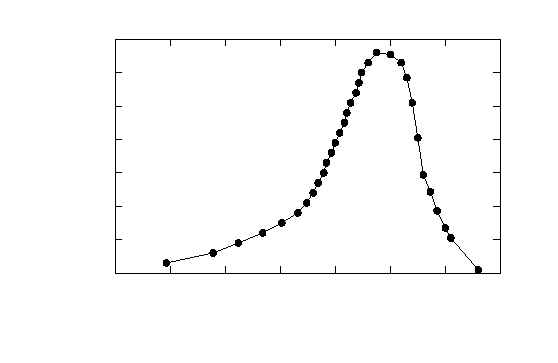
\includegraphics[width={252.00bp},height={158.40bp}]{silicon}}%
    \gplfronttext
  \end{picture}%
\endgroup
 }
        \captionsetup{type=graph}
        \caption{Spectral photovoltage dependence for silicon diode}
    \end{minipage} 
    \hfill
    \begin{minipage}[b]{.45\linewidth}
        \centering
        \resizebox{\textwidth}{!}{ % GNUPLOT: LaTeX picture with Postscript
\begingroup
  \makeatletter
  \providecommand\color[2][]{%
    \GenericError{(gnuplot) \space\space\space\@spaces}{%
      Package color not loaded in conjunction with
      terminal option `colourtext'%
    }{See the gnuplot documentation for explanation.%
    }{Either use 'blacktext' in gnuplot or load the package
      color.sty in LaTeX.}%
    \renewcommand\color[2][]{}%
  }%
  \providecommand\includegraphics[2][]{%
    \GenericError{(gnuplot) \space\space\space\@spaces}{%
      Package graphicx or graphics not loaded%
    }{See the gnuplot documentation for explanation.%
    }{The gnuplot epslatex terminal needs graphicx.sty or graphics.sty.}%
    \renewcommand\includegraphics[2][]{}%
  }%
  \providecommand\rotatebox[2]{#2}%
  \@ifundefined{ifGPcolor}{%
    \newif\ifGPcolor
    \GPcolorfalse
  }{}%
  \@ifundefined{ifGPblacktext}{%
    \newif\ifGPblacktext
    \GPblacktexttrue
  }{}%
  % define a \g@addto@macro without @ in the name:
  \let\gplgaddtomacro\g@addto@macro
  % define empty templates for all commands taking text:
  \gdef\gplbacktext{}%
  \gdef\gplfronttext{}%
  \makeatother
  \ifGPblacktext
    % no textcolor at all
    \def\colorrgb#1{}%
    \def\colorgray#1{}%
  \else
    % gray or color?
    \ifGPcolor
      \def\colorrgb#1{\color[rgb]{#1}}%
      \def\colorgray#1{\color[gray]{#1}}%
      \expandafter\def\csname LTw\endcsname{\color{white}}%
      \expandafter\def\csname LTb\endcsname{\color{black}}%
      \expandafter\def\csname LTa\endcsname{\color{black}}%
      \expandafter\def\csname LT0\endcsname{\color[rgb]{1,0,0}}%
      \expandafter\def\csname LT1\endcsname{\color[rgb]{0,1,0}}%
      \expandafter\def\csname LT2\endcsname{\color[rgb]{0,0,1}}%
      \expandafter\def\csname LT3\endcsname{\color[rgb]{1,0,1}}%
      \expandafter\def\csname LT4\endcsname{\color[rgb]{0,1,1}}%
      \expandafter\def\csname LT5\endcsname{\color[rgb]{1,1,0}}%
      \expandafter\def\csname LT6\endcsname{\color[rgb]{0,0,0}}%
      \expandafter\def\csname LT7\endcsname{\color[rgb]{1,0.3,0}}%
      \expandafter\def\csname LT8\endcsname{\color[rgb]{0.5,0.5,0.5}}%
    \else
      % gray
      \def\colorrgb#1{\color{black}}%
      \def\colorgray#1{\color[gray]{#1}}%
      \expandafter\def\csname LTw\endcsname{\color{white}}%
      \expandafter\def\csname LTb\endcsname{\color{black}}%
      \expandafter\def\csname LTa\endcsname{\color{black}}%
      \expandafter\def\csname LT0\endcsname{\color{black}}%
      \expandafter\def\csname LT1\endcsname{\color{black}}%
      \expandafter\def\csname LT2\endcsname{\color{black}}%
      \expandafter\def\csname LT3\endcsname{\color{black}}%
      \expandafter\def\csname LT4\endcsname{\color{black}}%
      \expandafter\def\csname LT5\endcsname{\color{black}}%
      \expandafter\def\csname LT6\endcsname{\color{black}}%
      \expandafter\def\csname LT7\endcsname{\color{black}}%
      \expandafter\def\csname LT8\endcsname{\color{black}}%
    \fi
  \fi
    \setlength{\unitlength}{0.0500bp}%
    \ifx\gptboxheight\undefined%
      \newlength{\gptboxheight}%
      \newlength{\gptboxwidth}%
      \newsavebox{\gptboxtext}%
    \fi%
    \setlength{\fboxrule}{0.5pt}%
    \setlength{\fboxsep}{1pt}%
    \definecolor{tbcol}{rgb}{1,1,1}%
\begin{picture}(5040.00,3168.00)%
    \gplgaddtomacro\gplbacktext{%
      \csname LTb\endcsname%%
      \put(814,704){\makebox(0,0)[r]{\strut{}$0$}}%
      \put(814,1078){\makebox(0,0)[r]{\strut{}$0.5$}}%
      \put(814,1452){\makebox(0,0)[r]{\strut{}$1$}}%
      \put(814,1826){\makebox(0,0)[r]{\strut{}$1.5$}}%
      \put(814,2199){\makebox(0,0)[r]{\strut{}$2$}}%
      \put(814,2573){\makebox(0,0)[r]{\strut{}$2.5$}}%
      \put(814,2947){\makebox(0,0)[r]{\strut{}$3$}}%
      \put(946,484){\makebox(0,0){\strut{}$0.6$}}%
      \put(1474,484){\makebox(0,0){\strut{}$0.8$}}%
      \put(2002,484){\makebox(0,0){\strut{}$1$}}%
      \put(2530,484){\makebox(0,0){\strut{}$1.2$}}%
      \put(3059,484){\makebox(0,0){\strut{}$1.4$}}%
      \put(3587,484){\makebox(0,0){\strut{}$1.6$}}%
      \put(4115,484){\makebox(0,0){\strut{}$1.8$}}%
      \put(4643,484){\makebox(0,0){\strut{}$2$}}%
    }%
    \gplgaddtomacro\gplfronttext{%
      \csname LTb\endcsname%%
      \put(209,1825){\rotatebox{-270}{\makebox(0,0){\strut{}$ U $ (mV) }}}%
      \put(2794,154){\makebox(0,0){\strut{} $\lambda \ \mu m $}}%
    }%
    \gplbacktext
    \put(0,0){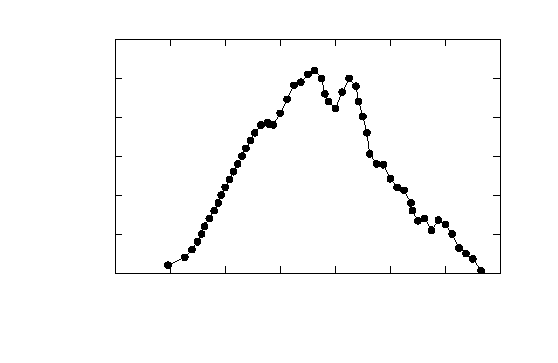
\includegraphics[width={252.00bp},height={158.40bp}]{germanium}}%
    \gplfronttext
  \end{picture}%
\endgroup
 }
        \captionsetup{type=graph}
        \caption{Spectral photovoltage dependence for germanium diode}
    \end{minipage} 
\end{table}

To also get the correct relative intensities of induced voltage, we need to divide by the relative intensity of light emitted by our lamp. The measured relative intensities can be seen in Table 3 and for the rest we will interpolate by a polynomial fit.

\begin{table}[htpb]
    \begin{minipage}[b]{.45\linewidth}
        \centering
        \begin{tabular}{c c c c}
            $ \lambda $ (nm) & D & $ \lambda $ (nm) & D \\ 
            \hline\hline
            1000 & 158 & 1500 & 110 \\
            1100 & 140 & 1600 & 95 \\
            1150 & 135 & 1700 & 70 \\
            1250 & 125 & 1800 & 46 \\
            1350 & 120 & 1850 & 35 \\
            1400 & 115 & 1900 & 15 \\
        \end{tabular}
        \caption{Relative intensities of light emitted by our lamp}

    \end{minipage} 
    \hfill
    \begin{minipage}[b]{.49\linewidth}
        \centering
        \resizebox{\textwidth}{!}{ % GNUPLOT: LaTeX picture with Postscript
\begingroup
  \makeatletter
  \providecommand\color[2][]{%
    \GenericError{(gnuplot) \space\space\space\@spaces}{%
      Package color not loaded in conjunction with
      terminal option `colourtext'%
    }{See the gnuplot documentation for explanation.%
    }{Either use 'blacktext' in gnuplot or load the package
      color.sty in LaTeX.}%
    \renewcommand\color[2][]{}%
  }%
  \providecommand\includegraphics[2][]{%
    \GenericError{(gnuplot) \space\space\space\@spaces}{%
      Package graphicx or graphics not loaded%
    }{See the gnuplot documentation for explanation.%
    }{The gnuplot epslatex terminal needs graphicx.sty or graphics.sty.}%
    \renewcommand\includegraphics[2][]{}%
  }%
  \providecommand\rotatebox[2]{#2}%
  \@ifundefined{ifGPcolor}{%
    \newif\ifGPcolor
    \GPcolorfalse
  }{}%
  \@ifundefined{ifGPblacktext}{%
    \newif\ifGPblacktext
    \GPblacktexttrue
  }{}%
  % define a \g@addto@macro without @ in the name:
  \let\gplgaddtomacro\g@addto@macro
  % define empty templates for all commands taking text:
  \gdef\gplbacktext{}%
  \gdef\gplfronttext{}%
  \makeatother
  \ifGPblacktext
    % no textcolor at all
    \def\colorrgb#1{}%
    \def\colorgray#1{}%
  \else
    % gray or color?
    \ifGPcolor
      \def\colorrgb#1{\color[rgb]{#1}}%
      \def\colorgray#1{\color[gray]{#1}}%
      \expandafter\def\csname LTw\endcsname{\color{white}}%
      \expandafter\def\csname LTb\endcsname{\color{black}}%
      \expandafter\def\csname LTa\endcsname{\color{black}}%
      \expandafter\def\csname LT0\endcsname{\color[rgb]{1,0,0}}%
      \expandafter\def\csname LT1\endcsname{\color[rgb]{0,1,0}}%
      \expandafter\def\csname LT2\endcsname{\color[rgb]{0,0,1}}%
      \expandafter\def\csname LT3\endcsname{\color[rgb]{1,0,1}}%
      \expandafter\def\csname LT4\endcsname{\color[rgb]{0,1,1}}%
      \expandafter\def\csname LT5\endcsname{\color[rgb]{1,1,0}}%
      \expandafter\def\csname LT6\endcsname{\color[rgb]{0,0,0}}%
      \expandafter\def\csname LT7\endcsname{\color[rgb]{1,0.3,0}}%
      \expandafter\def\csname LT8\endcsname{\color[rgb]{0.5,0.5,0.5}}%
    \else
      % gray
      \def\colorrgb#1{\color{black}}%
      \def\colorgray#1{\color[gray]{#1}}%
      \expandafter\def\csname LTw\endcsname{\color{white}}%
      \expandafter\def\csname LTb\endcsname{\color{black}}%
      \expandafter\def\csname LTa\endcsname{\color{black}}%
      \expandafter\def\csname LT0\endcsname{\color{black}}%
      \expandafter\def\csname LT1\endcsname{\color{black}}%
      \expandafter\def\csname LT2\endcsname{\color{black}}%
      \expandafter\def\csname LT3\endcsname{\color{black}}%
      \expandafter\def\csname LT4\endcsname{\color{black}}%
      \expandafter\def\csname LT5\endcsname{\color{black}}%
      \expandafter\def\csname LT6\endcsname{\color{black}}%
      \expandafter\def\csname LT7\endcsname{\color{black}}%
      \expandafter\def\csname LT8\endcsname{\color{black}}%
    \fi
  \fi
    \setlength{\unitlength}{0.0500bp}%
    \ifx\gptboxheight\undefined%
      \newlength{\gptboxheight}%
      \newlength{\gptboxwidth}%
      \newsavebox{\gptboxtext}%
    \fi%
    \setlength{\fboxrule}{0.5pt}%
    \setlength{\fboxsep}{1pt}%
    \definecolor{tbcol}{rgb}{1,1,1}%
\begin{picture}(4608.00,2880.00)%
    \gplgaddtomacro\gplbacktext{%
      \csname LTb\endcsname%%
      \put(814,704){\makebox(0,0)[r]{\strut{}$-50$}}%
      \put(814,1053){\makebox(0,0)[r]{\strut{}$0$}}%
      \put(814,1401){\makebox(0,0)[r]{\strut{}$50$}}%
      \put(814,1750){\makebox(0,0)[r]{\strut{}$100$}}%
      \put(814,2098){\makebox(0,0)[r]{\strut{}$150$}}%
      \put(814,2447){\makebox(0,0)[r]{\strut{}$200$}}%
      \put(1243,484){\makebox(0,0){\strut{}$1$}}%
      \put(1836,484){\makebox(0,0){\strut{}$1.2$}}%
      \put(2430,484){\makebox(0,0){\strut{}$1.4$}}%
      \put(3024,484){\makebox(0,0){\strut{}$1.6$}}%
      \put(3617,484){\makebox(0,0){\strut{}$1.8$}}%
      \put(4211,484){\makebox(0,0){\strut{}$2$}}%
    }%
    \gplgaddtomacro\gplfronttext{%
      \csname LTb\endcsname%%
      \put(209,1575){\rotatebox{-270}{\makebox(0,0){\strut{}D}}}%
      \put(2578,154){\makebox(0,0){\strut{} $\lambda \ \mu m $}}%
      \csname LTb\endcsname%%
      \put(3224,2274){\makebox(0,0)[r]{\strut{}fit}}%
    }%
    \gplbacktext
    \put(0,0){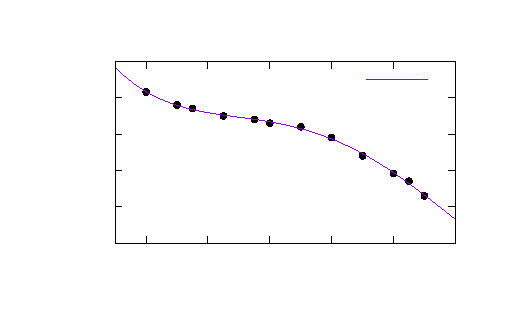
\includegraphics[width={230.40bp},height={144.00bp}]{cejchovani}}%
    \gplfronttext
  \end{picture}%
\endgroup
 }
        \captionsetup{type=graph}
        \caption{Fit of relative intensities from Table 3}
    \end{minipage} 
\end{table}

Unfortunately, our data points don't go all the way to the smallest measured wavelengths of $ 0.6 \ \mu m $. It is not a big problem though, since we are mainly interested in the peaks. Using equation (3) we get the following graphs

\begin{table}[htpb]
    \begin{minipage}[b]{.45\linewidth}
        \centering
        \resizebox{\textwidth}{!}{ % GNUPLOT: LaTeX picture with Postscript
\begingroup
  \makeatletter
  \providecommand\color[2][]{%
    \GenericError{(gnuplot) \space\space\space\@spaces}{%
      Package color not loaded in conjunction with
      terminal option `colourtext'%
    }{See the gnuplot documentation for explanation.%
    }{Either use 'blacktext' in gnuplot or load the package
      color.sty in LaTeX.}%
    \renewcommand\color[2][]{}%
  }%
  \providecommand\includegraphics[2][]{%
    \GenericError{(gnuplot) \space\space\space\@spaces}{%
      Package graphicx or graphics not loaded%
    }{See the gnuplot documentation for explanation.%
    }{The gnuplot epslatex terminal needs graphicx.sty or graphics.sty.}%
    \renewcommand\includegraphics[2][]{}%
  }%
  \providecommand\rotatebox[2]{#2}%
  \@ifundefined{ifGPcolor}{%
    \newif\ifGPcolor
    \GPcolorfalse
  }{}%
  \@ifundefined{ifGPblacktext}{%
    \newif\ifGPblacktext
    \GPblacktexttrue
  }{}%
  % define a \g@addto@macro without @ in the name:
  \let\gplgaddtomacro\g@addto@macro
  % define empty templates for all commands taking text:
  \gdef\gplbacktext{}%
  \gdef\gplfronttext{}%
  \makeatother
  \ifGPblacktext
    % no textcolor at all
    \def\colorrgb#1{}%
    \def\colorgray#1{}%
  \else
    % gray or color?
    \ifGPcolor
      \def\colorrgb#1{\color[rgb]{#1}}%
      \def\colorgray#1{\color[gray]{#1}}%
      \expandafter\def\csname LTw\endcsname{\color{white}}%
      \expandafter\def\csname LTb\endcsname{\color{black}}%
      \expandafter\def\csname LTa\endcsname{\color{black}}%
      \expandafter\def\csname LT0\endcsname{\color[rgb]{1,0,0}}%
      \expandafter\def\csname LT1\endcsname{\color[rgb]{0,1,0}}%
      \expandafter\def\csname LT2\endcsname{\color[rgb]{0,0,1}}%
      \expandafter\def\csname LT3\endcsname{\color[rgb]{1,0,1}}%
      \expandafter\def\csname LT4\endcsname{\color[rgb]{0,1,1}}%
      \expandafter\def\csname LT5\endcsname{\color[rgb]{1,1,0}}%
      \expandafter\def\csname LT6\endcsname{\color[rgb]{0,0,0}}%
      \expandafter\def\csname LT7\endcsname{\color[rgb]{1,0.3,0}}%
      \expandafter\def\csname LT8\endcsname{\color[rgb]{0.5,0.5,0.5}}%
    \else
      % gray
      \def\colorrgb#1{\color{black}}%
      \def\colorgray#1{\color[gray]{#1}}%
      \expandafter\def\csname LTw\endcsname{\color{white}}%
      \expandafter\def\csname LTb\endcsname{\color{black}}%
      \expandafter\def\csname LTa\endcsname{\color{black}}%
      \expandafter\def\csname LT0\endcsname{\color{black}}%
      \expandafter\def\csname LT1\endcsname{\color{black}}%
      \expandafter\def\csname LT2\endcsname{\color{black}}%
      \expandafter\def\csname LT3\endcsname{\color{black}}%
      \expandafter\def\csname LT4\endcsname{\color{black}}%
      \expandafter\def\csname LT5\endcsname{\color{black}}%
      \expandafter\def\csname LT6\endcsname{\color{black}}%
      \expandafter\def\csname LT7\endcsname{\color{black}}%
      \expandafter\def\csname LT8\endcsname{\color{black}}%
    \fi
  \fi
    \setlength{\unitlength}{0.0500bp}%
    \ifx\gptboxheight\undefined%
      \newlength{\gptboxheight}%
      \newlength{\gptboxwidth}%
      \newsavebox{\gptboxtext}%
    \fi%
    \setlength{\fboxrule}{0.5pt}%
    \setlength{\fboxsep}{1pt}%
    \definecolor{tbcol}{rgb}{1,1,1}%
\begin{picture}(5040.00,3168.00)%
    \gplgaddtomacro\gplbacktext{%
      \csname LTb\endcsname%%
      \put(550,704){\makebox(0,0)[r]{\strut{}$0$}}%
      \put(550,984){\makebox(0,0)[r]{\strut{}$1$}}%
      \put(550,1265){\makebox(0,0)[r]{\strut{}$2$}}%
      \put(550,1545){\makebox(0,0)[r]{\strut{}$3$}}%
      \put(550,1826){\makebox(0,0)[r]{\strut{}$4$}}%
      \put(550,2106){\makebox(0,0)[r]{\strut{}$5$}}%
      \put(550,2386){\makebox(0,0)[r]{\strut{}$6$}}%
      \put(550,2667){\makebox(0,0)[r]{\strut{}$7$}}%
      \put(550,2947){\makebox(0,0)[r]{\strut{}$8$}}%
      \put(682,484){\makebox(0,0){\strut{}$1$}}%
      \put(1342,484){\makebox(0,0){\strut{}$1.2$}}%
      \put(2002,484){\makebox(0,0){\strut{}$1.4$}}%
      \put(2662,484){\makebox(0,0){\strut{}$1.6$}}%
      \put(3323,484){\makebox(0,0){\strut{}$1.8$}}%
      \put(3983,484){\makebox(0,0){\strut{}$2$}}%
      \put(4643,484){\makebox(0,0){\strut{}$2.2$}}%
    }%
    \gplgaddtomacro\gplfronttext{%
      \csname LTb\endcsname%%
      \put(209,1825){\rotatebox{-270}{\makebox(0,0){\strut{}S}}}%
      \put(2662,154){\makebox(0,0){\strut{}E (eV)}}%
    }%
    \gplbacktext
    \put(0,0){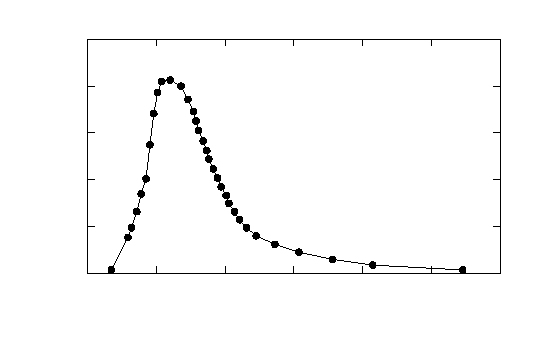
\includegraphics[width={252.00bp},height={158.40bp}]{silicon_S}}%
    \gplfronttext
  \end{picture}%
\endgroup
 }
        \captionsetup{type=graph}
        \caption{Spectral dependence of photon energy for silicon diode }
    \end{minipage} 
    \hfill
    \begin{minipage}[b]{.45\linewidth}
        \centering
        \resizebox{\textwidth}{!}{ % GNUPLOT: LaTeX picture with Postscript
\begingroup
  \makeatletter
  \providecommand\color[2][]{%
    \GenericError{(gnuplot) \space\space\space\@spaces}{%
      Package color not loaded in conjunction with
      terminal option `colourtext'%
    }{See the gnuplot documentation for explanation.%
    }{Either use 'blacktext' in gnuplot or load the package
      color.sty in LaTeX.}%
    \renewcommand\color[2][]{}%
  }%
  \providecommand\includegraphics[2][]{%
    \GenericError{(gnuplot) \space\space\space\@spaces}{%
      Package graphicx or graphics not loaded%
    }{See the gnuplot documentation for explanation.%
    }{The gnuplot epslatex terminal needs graphicx.sty or graphics.sty.}%
    \renewcommand\includegraphics[2][]{}%
  }%
  \providecommand\rotatebox[2]{#2}%
  \@ifundefined{ifGPcolor}{%
    \newif\ifGPcolor
    \GPcolorfalse
  }{}%
  \@ifundefined{ifGPblacktext}{%
    \newif\ifGPblacktext
    \GPblacktexttrue
  }{}%
  % define a \g@addto@macro without @ in the name:
  \let\gplgaddtomacro\g@addto@macro
  % define empty templates for all commands taking text:
  \gdef\gplbacktext{}%
  \gdef\gplfronttext{}%
  \makeatother
  \ifGPblacktext
    % no textcolor at all
    \def\colorrgb#1{}%
    \def\colorgray#1{}%
  \else
    % gray or color?
    \ifGPcolor
      \def\colorrgb#1{\color[rgb]{#1}}%
      \def\colorgray#1{\color[gray]{#1}}%
      \expandafter\def\csname LTw\endcsname{\color{white}}%
      \expandafter\def\csname LTb\endcsname{\color{black}}%
      \expandafter\def\csname LTa\endcsname{\color{black}}%
      \expandafter\def\csname LT0\endcsname{\color[rgb]{1,0,0}}%
      \expandafter\def\csname LT1\endcsname{\color[rgb]{0,1,0}}%
      \expandafter\def\csname LT2\endcsname{\color[rgb]{0,0,1}}%
      \expandafter\def\csname LT3\endcsname{\color[rgb]{1,0,1}}%
      \expandafter\def\csname LT4\endcsname{\color[rgb]{0,1,1}}%
      \expandafter\def\csname LT5\endcsname{\color[rgb]{1,1,0}}%
      \expandafter\def\csname LT6\endcsname{\color[rgb]{0,0,0}}%
      \expandafter\def\csname LT7\endcsname{\color[rgb]{1,0.3,0}}%
      \expandafter\def\csname LT8\endcsname{\color[rgb]{0.5,0.5,0.5}}%
    \else
      % gray
      \def\colorrgb#1{\color{black}}%
      \def\colorgray#1{\color[gray]{#1}}%
      \expandafter\def\csname LTw\endcsname{\color{white}}%
      \expandafter\def\csname LTb\endcsname{\color{black}}%
      \expandafter\def\csname LTa\endcsname{\color{black}}%
      \expandafter\def\csname LT0\endcsname{\color{black}}%
      \expandafter\def\csname LT1\endcsname{\color{black}}%
      \expandafter\def\csname LT2\endcsname{\color{black}}%
      \expandafter\def\csname LT3\endcsname{\color{black}}%
      \expandafter\def\csname LT4\endcsname{\color{black}}%
      \expandafter\def\csname LT5\endcsname{\color{black}}%
      \expandafter\def\csname LT6\endcsname{\color{black}}%
      \expandafter\def\csname LT7\endcsname{\color{black}}%
      \expandafter\def\csname LT8\endcsname{\color{black}}%
    \fi
  \fi
    \setlength{\unitlength}{0.0500bp}%
    \ifx\gptboxheight\undefined%
      \newlength{\gptboxheight}%
      \newlength{\gptboxwidth}%
      \newsavebox{\gptboxtext}%
    \fi%
    \setlength{\fboxrule}{0.5pt}%
    \setlength{\fboxsep}{1pt}%
    \definecolor{tbcol}{rgb}{1,1,1}%
\begin{picture}(5040.00,3168.00)%
    \gplgaddtomacro\gplbacktext{%
      \csname LTb\endcsname%%
      \put(550,704){\makebox(0,0)[r]{\strut{}$0$}}%
      \put(550,1024){\makebox(0,0)[r]{\strut{}$1$}}%
      \put(550,1345){\makebox(0,0)[r]{\strut{}$2$}}%
      \put(550,1665){\makebox(0,0)[r]{\strut{}$3$}}%
      \put(550,1986){\makebox(0,0)[r]{\strut{}$4$}}%
      \put(550,2306){\makebox(0,0)[r]{\strut{}$5$}}%
      \put(550,2627){\makebox(0,0)[r]{\strut{}$6$}}%
      \put(550,2947){\makebox(0,0)[r]{\strut{}$7$}}%
      \put(682,484){\makebox(0,0){\strut{}$0.6$}}%
      \put(1078,484){\makebox(0,0){\strut{}$0.7$}}%
      \put(1474,484){\makebox(0,0){\strut{}$0.8$}}%
      \put(1870,484){\makebox(0,0){\strut{}$0.9$}}%
      \put(2266,484){\makebox(0,0){\strut{}$1$}}%
      \put(2663,484){\makebox(0,0){\strut{}$1.1$}}%
      \put(3059,484){\makebox(0,0){\strut{}$1.2$}}%
      \put(3455,484){\makebox(0,0){\strut{}$1.3$}}%
      \put(3851,484){\makebox(0,0){\strut{}$1.4$}}%
      \put(4247,484){\makebox(0,0){\strut{}$1.5$}}%
      \put(4643,484){\makebox(0,0){\strut{}$1.6$}}%
    }%
    \gplgaddtomacro\gplfronttext{%
      \csname LTb\endcsname%%
      \put(209,1825){\rotatebox{-270}{\makebox(0,0){\strut{}S}}}%
      \put(2662,154){\makebox(0,0){\strut{}E (eV)}}%
    }%
    \gplbacktext
    \put(0,0){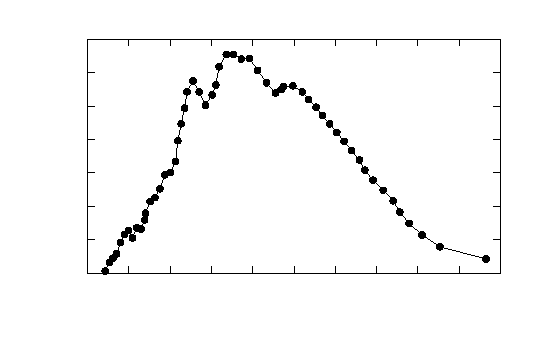
\includegraphics[width={252.00bp},height={158.40bp}]{germanium_S}}%
    \gplfronttext
  \end{picture}%
\endgroup
 }
        \captionsetup{type=graph}
        \caption{Spectral dependence of photon energy for germanium diode }
    \end{minipage} 
\end{table}


\section{Conclusion}

We've measured the spectral dependence of photovoltage induced by a monochromatic beam of light on PN junctions of a germanium and silicon diode which is shown in Graphs 1 and 2. A~measured voltage was only seen from the wavelength $ \lambda = 1160 $ nm for silicon and $ \lambda = 1930 $ nm, from which we conclude that the corresponding band gap energies are $ E_g = 1.069 $ eV and $ E_g = 0.642 $~eV respectively. Table values give $ E_g = 1.12 $ eV and $ E = 0.67 $ eV, which is not a bad result. The slight differences are likely due to measurement inaccuracies on my part.

Our measured voltages were not completely to scale since the source of light did not emit light at even intensities. We've adjusted for this difference using measured relative intensity of the halogen lamp and plotted the corrected Graphs 4 and 5. It can be seen, that both follow a similar shape of one peek, but in the case of germanium there are significant dips at specific wavelengths. It seems like there are other ways of absorbing the photons which only come to effect at those specific wave lengths and reduce the induced voltage. 

\begin{thebibliography}{0}
\bibitem{tabulky} Task instructions ~\url{https://is.muni.cz/auth/el/sci/jaro2025/F4210/um/fp3-8_sirka_pasu.pdf}.   
\end{thebibliography}

%\begin{table}[htpb]
%    \scriptsize
%    \begin{minipage}{.4\linewidth}
%    \centering
%    \begin{tabular}{| c c | c c |}
%        \hline
%        $ \lambda $ (nm) & $ U_m $ (mV) & $ \lambda $ (nm) & $ U_m $ (mV) \\
%        \hline
%        593 & 0.03 &  948 & 0.60 \\
%        678 & 0.06 &  960 & 0.63 \\
%        724 & 0.09 &  975 & 0.66 \\
%        768 & 0.12 & 1000 & 0.65 \\
%        803 & 0.15 & 1020 & 0.63 \\
%        832 & 0.18 & 1030 & 0.59 \\
%        848 & 0.21 & 1040 & 0.51 \\
%        860 & 0.24 & 1050 & 0.41 \\
%        869 & 0.27 & 1060 & 0.29 \\
%        879 & 0.30 & 1073 & 0.24 \\
%        884 & 0.33 & 1085 & 0.19 \\
%        893 & 0.36 & 1100 & 0.14 \\
%        900 & 0.39 & 1110 & 0.11 \\
%        908 & 0.42 & 1160 & 0.01 \\
%        917 & 0.45 & & \\
%        921 & 0.48 & & \\
%        928 & 0.51 & & \\
%        938 & 0.54 & & \\
%        943 & 0.57 & & \\
%        \hline
%    \end{tabular}
%    \caption{Measured spectral photovoltage dependence of silicon diode.}
%    \end{minipage} 
%    \hfill
%    \begin{minipage}{.55\linewidth}
%    \centering
%    \begin{tabular}{| c c | c c | c c |}
%        \hline
%        $ \lambda $ (nm) & $ U_m $ (mV) & $ \lambda $ (nm) & $ U_m $ (mV) & $ \lambda $ (nm) & $ U_m $ (mV) \\
%        \hline
%        0.792 & 0.030 & 1.154 & 0.579 & 1.525 & 0.459 \\
%        0.853 & 0.060 & 1.160 & 0.573 & 1.550 & 0.420 \\
%        0.879 & 0.090 & 1.175 & 0.570 & 1.575 & 0.417 \\
%        0.899 & 0.120 & 1.200 & 0.615 & 1.600 & 0.363 \\
%        0.914 & 0.150 & 1.225 & 0.669 & 1.625 & 0.330 \\
%        0.925 & 0.180 & 1.250 & 0.723 & 1.650 & 0.318 \\
%        0.942 & 0.210 & 1.275 & 0.735 & 1.675 & 0.270 \\
%        0.960 & 0.240 & 1.300 & 0.765 & 1.680 & 0.240 \\
%        0.975 & 0.270 & 1.325 & 0.780 & 1.700 & 0.201 \\
%        0.985 & 0.300 & 1.350 & 0.750 & 1.725 & 0.210 \\
%        1.000 & 0.330 & 1.362 & 0.690 & 1.750 & 0.165 \\
%        1.015 & 0.360 & 1.375 & 0.660 & 1.775 & 0.204 \\
%        1.030 & 0.390 & 1.400 & 0.633 & 1.800 & 0.186 \\
%        1.045 & 0.420 & 1.425 & 0.696 & 1.825 & 0.150 \\
%        1.061 & 0.450 & 1.450 & 0.750 & 1.850 & 0.096 \\
%        1.075 & 0.480 & 1.475 & 0.720 & 1.875 & 0.075 \\
%        1.092 & 0.510 & 1.485 & 0.660 & 1.900 & 0.054 \\
%        1.107 & 0.540 & 1.500 & 0.603 & 1.930 & 0.009 \\
%        1.130 & 0.570 & 1.515 & 0.540 & & \\
%        \hline
%    \end{tabular}
%    \caption{Measured spectral photovoltage dependence of germanium diode.}
%    \end{minipage} 
%\end{table}

 

\end{document}
